\documentclass[../main.tex]{subfiles}
\begin{document}
\section{Results}
%---------------------------------------------------
\subsection{$2 \times 2$ lattice, analytical expressions}
If we scale the value of $\beta$ from $1/k_BT$ to $1/J$ (Scaling factor $k_B T/J$) in the analytical expression from section \ref{sec:theory-analy}, we will get a good benchmark for computer computations to come. These values are listed in table \ref{tab:2x2spinsEnergiesMags} below. Note that all values are divided by four, since we want the values per bond, and not for the entire lattice.
\begin{table}[!h]
\begin{center}
  \begin{tabular}{| l | r |}
    \hline
    \textbf{Mean energy,} $\mathbf{\langle E \rangle}$ & $-1.9960$  \\
    \hline
    \textbf{Mean absolute magnetization,} $\mathbf{\langle |\mathcal{M}| \rangle}$ & $0.9987$ \\
    \hline
    \textbf{Specific heat capacity,} $\mathbf{C_V}$ & $0.0321$\\
    \hline
    \textbf{Susceptibility,} $\mathbf \chi$ & $3.9933$ \\
    \hline
  \end{tabular}
  \caption{Analytically calculated benchmark for material characteristics per bond for a $2 \times 2$ lattice}
  \label{tab:2x2spinsEnergiesMags}
\end{center}
\end{table}
\FloatBarrier

\subsection{$2 \times 2$ lattice, numerical results}
Using $T = 1.0$, like in the analytical calculations, the program \href{https://github.com/kmaasrud/Project-4/tree/master/code/Ising}{/code/Ising/} gives the results listed in table \ref{tab:2x2computed}:
\begin{table}[!h]
  \begin{center}
    \begin{tabular}{| l | r | r |}
      \hline
       & \textbf{Set initialization} & \textbf{Random initialization} \\
      \hline
      \textbf{Mean energy,} $\mathbf{\langle E \rangle}$ & $-1.9955$ & $-1.9958$\\
      \hline
      \textbf{Mean absolute magnetization,} $\mathbf{\langle |\mathcal{M}| \rangle}$ & $0.9985$ & $0.9986$ \\
      \hline
      \textbf{Specific heat capacity,} $\mathbf{C_v}$ & $0.0358$ & $0.0337$ \\
      \hline
      \textbf{Susceptibility,} $\mathbf \chi$ & $3.9925$ & $3.8237$ \\
      \hline
    \end{tabular}
    \caption{Computed values of material characteristics per bond for a $2\times 2$ lattice.}
    \label{tab:2x2computed}
  \end{center}
\end{table}
\FloatBarrier
The values correspond very well with each other and the analytical.

%---------------------------------------------------
\subsection{Ising model: simulation over temperature} \label{sec:res-compareanalytical}
We ran the program for different amounts of Monte Carlo cycles and plotted the error ($\text{analytical} - \text{simulated}$) in figure \ref{fig:results-MCplot} below. Using $10^7$ Monte Carlo cycles, we seem to be getting pretty accurate results.

\begin{figure}[!h]
  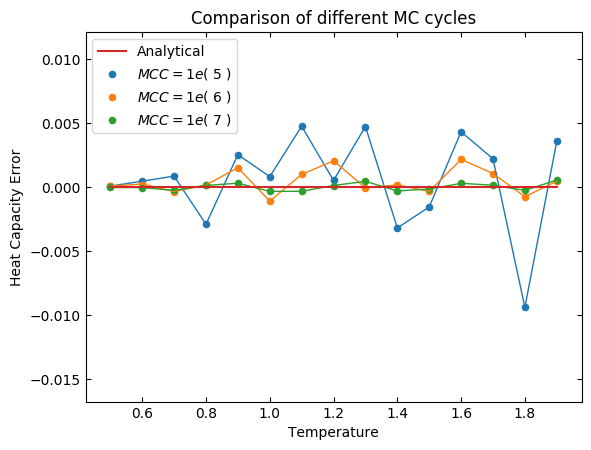
\includegraphics[scale=0.7]{CyclesComparison.png}
  \caption{Shows the accuracy of different amount of MC cycles over temperature.}
  \label{fig:results-MCplot}
\end{figure}
\FloatBarrier
This shows that our computed results are quite close to our analytical results for the $20\times 20$ lattice. This is a good indication of a successfull simulation.
%---------------------------------------------------
\subsection{$20 \times 20$ lattice} \label{sec:results-20x20lattice}
%---------------------------------------------------
\subsubsection*{Ordered spin orientation}
Initializing the spin structure, we first set every spin up for $T<1.5$ and every spin down for $T\ge 1.5$. In figure \ref{fig:ordered}, the computed values for the mean magnetization and energy are plotted against the number of MC cycles, at $T=1.0$ and $T=2.4$:

\begin{figure}[!h]
  \centering
  \makebox[\textwidth][c]{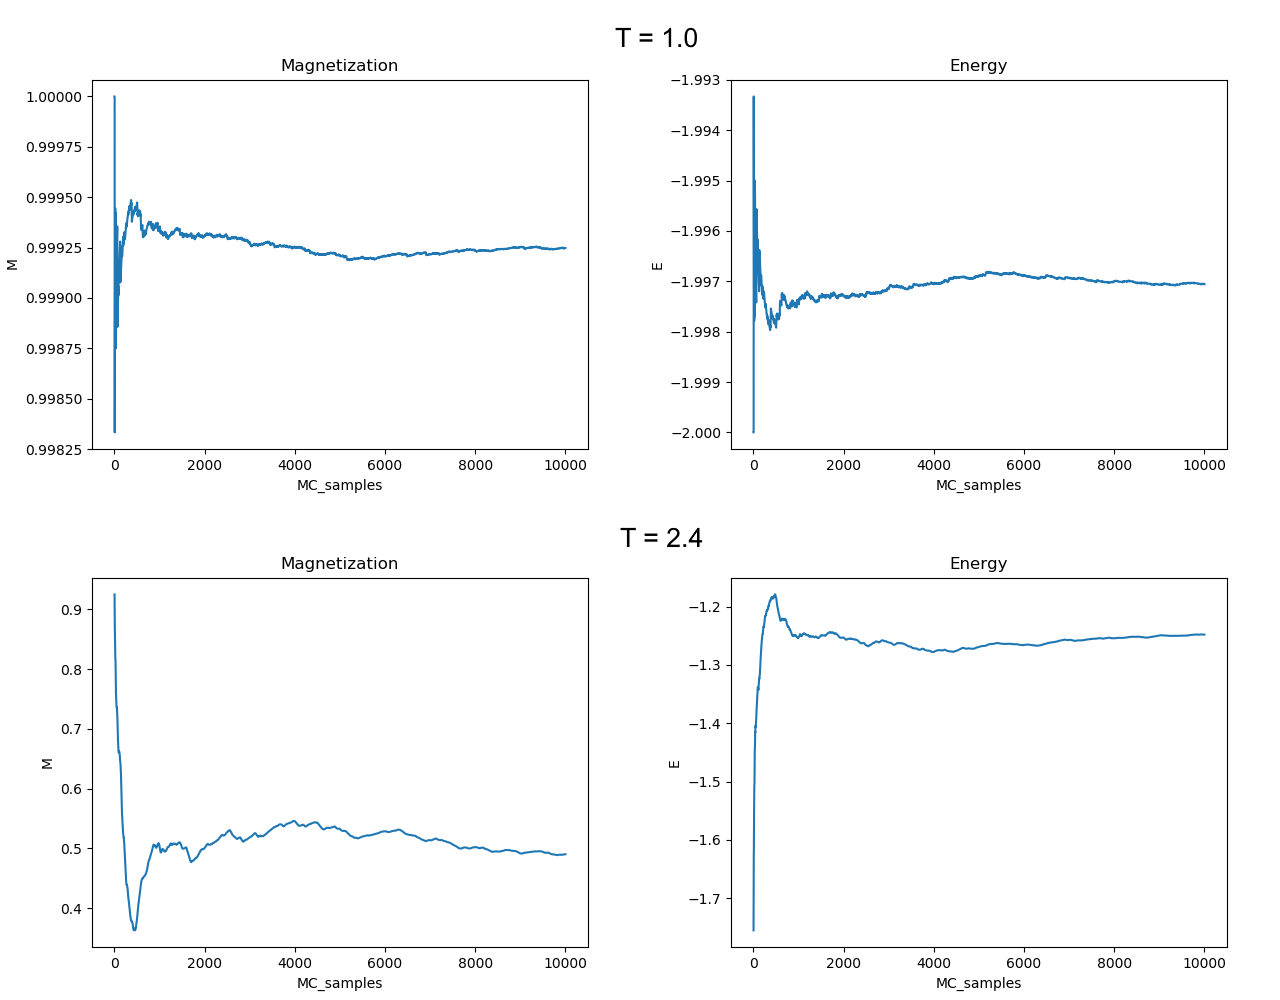
\includegraphics[width=1.3\textwidth]{./M+E/ordered.png}}
  \caption{Shows the computed value for the mean magnetization and energy, with ordered initialization, against the number of MC cycles. The scaled temperature is $T=1.0$ and $T=2.4$ respectively.}
  \label{fig:ordered}
\end{figure}
\FloatBarrier
All the plots pretty much stabilize into a value after 8000-1000 MC cycles. For $T=1.0$, the magnetization stabilizes around the value $0.99950$ and the energy around the value $-1.997$. This corresponds pretty good with the analytically calculated values. For $T=2.4$, the magnetization stabilizes around the value $0.5$ and the energy around the value $-1.25$.

%---------------------------------------------------
\subsubsection*{Random spin orientation}
Following the ordered initialisation, we also initialized the crystal randomly. In figure \ref{fig:random}, the computed values for the mean magnetization and energy are plotted against the number of MC cycles, at $T=1.0$ and $T=2.4$:

\begin{figure}[!h]
  \centering
  \makebox[\textwidth][c]{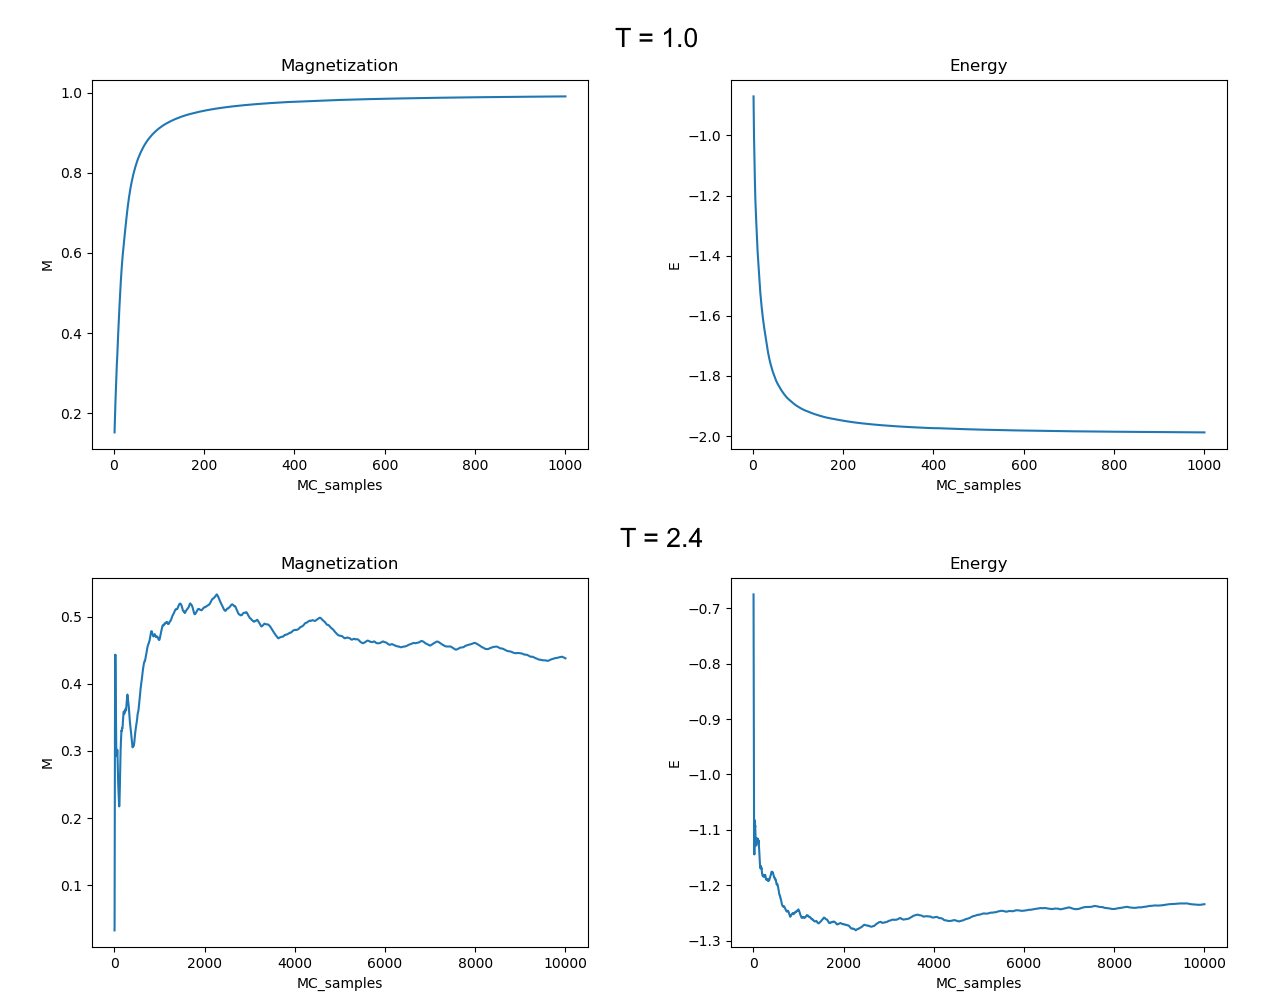
\includegraphics[width=1.3\textwidth]{./M+E/random.png}}
  \caption{Shows the computed value for the mean magnetization and energy, with random initialization, against the number of MC cycles. The scaled temperature is $T=1.0$ and $T=2.4$ respectively.}
  \label{fig:random}
\end{figure}
\FloatBarrier
The plots for $T=1.0$ follow a clean exponential curve, while the other plots pretty much stabilize after 8000-1000 MC cycles - like the previous ones. For $T=1.0$, the magnetization ends on the value $1.0$ and the energy on the value $-2.0$. This is similar to the analytical values, but does not have the same accuracy. For $T=2.4$, the magnetization stabilizes around the value $0.45$ and the energy around the value $-1.25$.
% Tekst: Random spinn orientering for T = 1.0

% Likevekt ved:
% T = 2.4(kT/J):
% Mean energy and magnetization func of MC cycles:
% Ordnet orientering: Program initilize.cpp (For T < 1.5 så er alle spinn opp,
% ellers spinn ned)
% Tekst: ordnet spinn orientering for T= 2.4
% Random spinn orientering: Program initilize_random (Setter spinn ned(-1)
% hvis verdien vi får mellom 0 og 1 er mindre eller lik 0.5 ).
% Tekst: Random spinn orientering for T = 2.4


% Likevekt ved:

% Oversiktelig tabell med når likevekt nås ca. (antall mcs)

%     Ordnet magnetisering  Random magnetisering  Ordnet energi Random energi
% T1:
% T2:

% Estimat av equilibration time:


% Antall aksepterte spinn totalt etter et gitt antall mcs(100k maks):
% Set start point
% T = 1

% Bilde :accepted_spinn_T1_mcs_cumsum(y)_log10.png
% Stabiliserer seg ved mcd = 1E3.5(alle spinn blir heretter akseptert)
%
% T = 2.4
% Bilde: accepted_spinn_T2_mcs_cumsum(y)_log10.png
% Stabiliserer seg ved mcd = 1E3.5, men det er mange flere som blir akseptert(Se y aksen)
%
%
%
% Random start point:
% T = 1:
% Bilde: accepted_spins_T1_random_cumsum(y)_mcs_log10.png
% T = 2.4
% Bilde: accepted_spins_T2_random_cumsum(y)_mcs_log10.png
%
% Temperaturavhengighet(skal vi lage plot her også- eller holder det med kommentar i resultater?):
% Økt temperatur gjør at mange flere spinn aksepteres ved lavere antall mcs dvs tidligere.(sjekk prosenten på y aksen)
% Ved random vs ikke random: omtrent like mange som aksepteres, men i random så aksepteres flere spinn ved lavere mcs. Ved T1 random får man en liten økning ved 1E1.5, mens hos T1 set startpont så før vi ikke en økning i aksepterte spinn før ved 1E3.5
%
% For T2 så får vi økningen på samme sted dvs 1E4 på både random og satt startpunkt.

% Diskusjon/resultater
% Aksepterte spinn som funksjon av T:
% Økt temperatur gir flere aksepterte flips.
% Setter man startpoint til random går den fortere mot likevekt ?

\subsection{Analyzing the probability distribution}
In figure \ref{fig:results-ProbE_T24} you can see the probability distribution for low and high temperature respectively. We can see that for a low temperature, the system tends to settle in the lowest energy state, while for the higher temperature the energies are a bit more spread. In table \ref{tab:results-variance} you will see the computed variance. Note that we calculated standard deviation of the histogram with \textsc{numpy.std}, and took the square root of this to get the variance.

\begin{figure}[!h]
  \centering
  \makebox[\textwidth][c]{
  \begin{minipage}{0.7\textwidth}
        \centering
        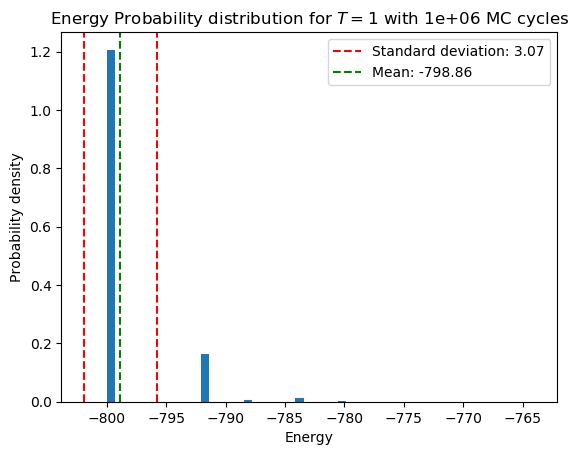
\includegraphics[width=1\textwidth]{ProbE_T1.png} % first figure itself
    \end{minipage}\hfill
    \begin{minipage}{0.7\textwidth}
        \centering
        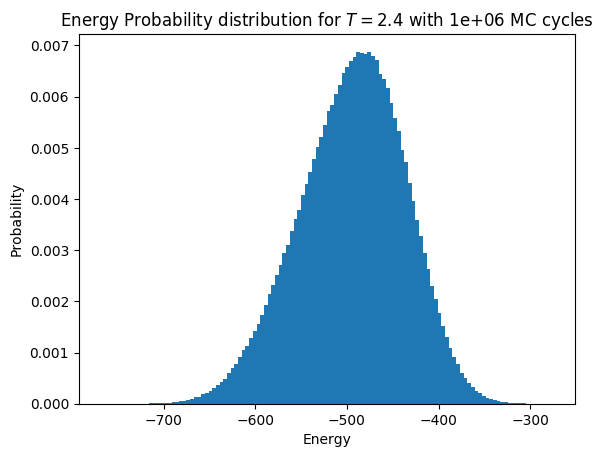
\includegraphics[width=1\textwidth]{ProbE_T24.png} % second figure itself
    \end{minipage}
}
  \caption{Shows probability distribution for low and high temperature.}
  \label{fig:results-ProbE_T24}
\end{figure}
\FloatBarrier


\begin{table}[!h]
  \begin{center}
    \begin{tabular}{|l| l| l| l|}
      \hline
      Temperature & calculated variance & from histogram & deviation\\
      \hline
      1 & 9.375 & 1.752 & 81\%\\
      2.4 & 8.053  & 7.550 & 6.2\%\\
      \hline
    \end{tabular}
    \caption{Computed variance}
    \label{tab:results-variance}
  \end{center}
\end{table}
\FloatBarrier

%---------------------------------------------------
\subsection{Numerical studies of phase transitions}
After playing around with the domain of the temperature we found that the domain used in figure \ref{fig:results-energy-magnetisation} and \ref{fig:results-heatcap-suscep} nicely presents the phase change of the material. We used $10^6$ Monte Carlo Cycles for each temperature step, which had a stepsize of $\Delta T = 0.005$. As shown in the figures we can clearly see that something is happening around $T = 2.3$.

\begin{figure}[!h]
\makebox[\textwidth][c]{
  \begin{minipage}[t]{0.7\textwidth}
    \centering
    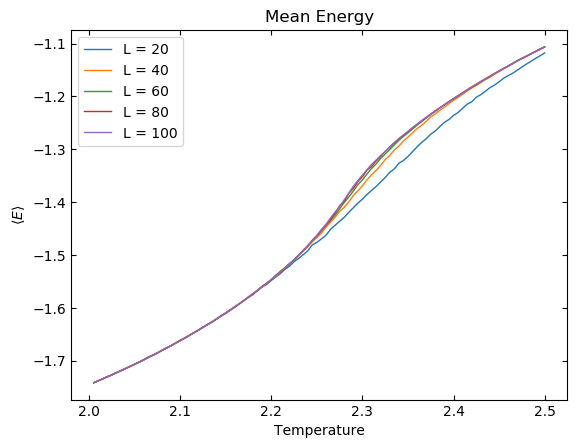
\includegraphics[width=1\textwidth]{eEnergy.png}

  \end{minipage}

  \begin{minipage}[t]{0.7\textwidth}
    \centering
    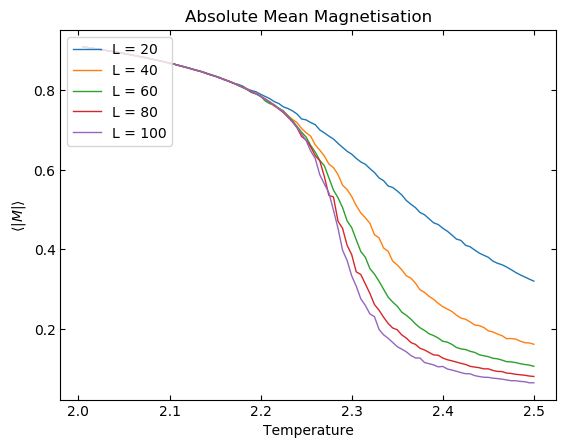
\includegraphics[width=1\textwidth]{eMagnetisation.png}

  \end{minipage}
  }
  \caption{Mean energy and magnetisation over temperature interval $T \in [2.0, 2.5]$ with lattice sizes $L = {20, 40, 60, 80, 100}$.}
  \label{fig:results-energy-magnetisation}
\end{figure}
\FloatBarrier

\begin{figure}[!h]
\makebox[\textwidth][c]{
  \begin{minipage}[t]{0.7\textwidth}
    \centering
    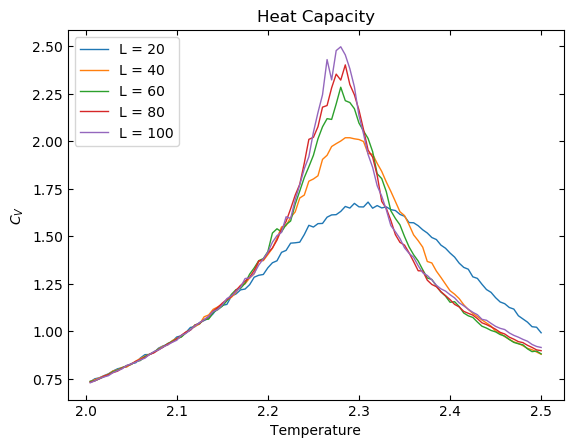
\includegraphics[width=1\textwidth]{eHeatcapacity.png}

  \end{minipage}

  \begin{minipage}[t]{0.7\textwidth}
    \centering
    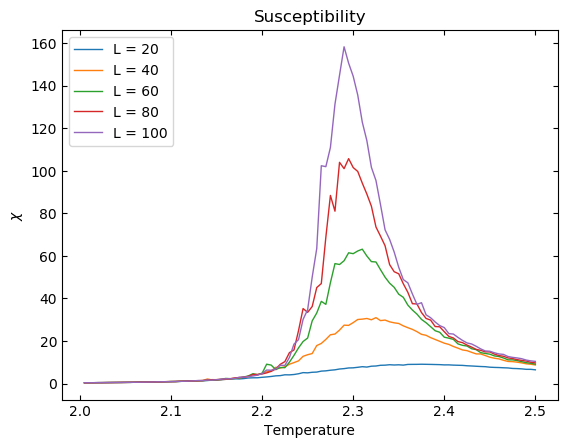
\includegraphics[width=1\textwidth]{eSusceptibility.png}

  \end{minipage}
  }
  \caption{Heat capacity and Susceptibility over temperature interval $T \in [2.0, 2.5]$ with lattice sizes $L = {20, 40, 60, 80, 100}$.}
  \label{fig:results-heatcap-suscep}
\end{figure}
\FloatBarrier
The simulations were run on an 16-core AMD Ryzen 1700x with 3.4GHz clock speed. It took approximately 3 hours to complete.\\
To compare parallelized time to using a single core, we ran calculations for the 20x20 lattice with $10^5$ Monte Carlo cycles and $T \in [2.0, 2.5]$ with step size $\Delta T = 0.05$. The time is shown in table \ref{tab:results-MPI}.

\begin{table}[!h]
  \begin{center}
    \begin{tabular}{|c| l|}
      \hline
      Cores & Time spent\\
      \hline
      1 & 42s\\
      2 & 26s\\
      \hline
    \end{tabular}
    \caption{Time spent on calculations for different thread-count.}
    \label{tab:results-MPI}
  \end{center}
\end{table}
\FloatBarrier

%---------------------------------------------------

\subsection{Extracting the critical temperature}
The critical temperatures of the different sized arrays was found by taking the averange of the full width half maximum of the heat capacity and the susceptibility. This resulted in the critical temperatures found in table \ref{tab:results-TC-lattices}.
\begin{table}[!h]
  \begin{center}
    \begin{tabular}{|c| l|}
      \hline
      Lattice size, L & $T_C$ \\
      \hline
      40 & 2.318\\
      60 & 2.301\\
      80 & 2.291\\
      100 & 2.284\\
      \hline
    \end{tabular}
    \caption{Critical temperatures of different lattice sizes.}
    \label{tab:results-TC-lattices}
  \end{center}
\end{table}
\FloatBarrier
By using equation \eqref{eq:a}, and \eqref{eq:TC}. we find the constant a, and thereafter the critical temperature for an infinitely large lattice.

\begin{table}[!h]
  \begin{center}
    \begin{tabular}{|c| l|}
      \hline
      Parameter & Value \\
      \hline
      a & 2.26667\\
      $T_C$ & 2.261\\
      \hline
    \end{tabular}
    \caption{Numerical values for the parameter a, and the critical temperature.}
    \label{tab:results-a-and-TC}
  \end{center}
\end{table}
\FloatBarrier

For reference, the exact result for the criticalt temperature for $L \rightarrow \infty$ is $kT/J = 2/ln(1 +\sqrt{2}) \approx 2.269$ after Lars Onsager.\cite{larsonsager}

\end{document}
